	\section{REPULSION}
	\hspace{1cm}{\large Preventing Entry and Establishing Defensive Barriers}
	
	\subsection{The Core Logic}
	\paragraph{}
	The Ars Goetia operates on a hierarchy of names and symbols that assert divine authority over all 72 spirits.  The generalized elements are more powerful than individual spirit sigils because they invoke the source of authority rather than targeting an individual entity.  It is like having a master key instead of 72 separate keys.
	
	\subsection{Universal Names of Compulsion}
	These names from the Goetic conjurations work against all spirits of the hierarchy:
	
\begin{flushleft}
	\begin{xltabular}{\textwidth}{|l|X|}
		\hline
		\textbf{Name} & \textbf{Function} \\ \hline
		\endfirsthead
		\hline
		\textbf{Name} & \textbf{Function} \\ \hline
		\endhead
		
		TETRAGRAMMATON & Supreme divine authority (YHVH) \\ \hline
		ADONAI & Lordship and mastery \\ \hline
		AGLA & Protective barrier ("Thou art mighty forever, O Lord") \\ \hline
		PRIMEUMATON & First cause?commands origin \\ \hline
		ANAPHAXETON & Binds the hidden and formless \\ \hline
		EHYEH & "I Am" ? self?existent divine presence \\ \hline
		EL & God (generic, universal) \\ \hline
		ON & Being itself \\ \hline
		\caption{Universal Names of Compulsion}
		
	\end{xltabular}
\end{flushleft}

	\subsection{The Circle of Solomon}
	The original Circle of Solomon serves as the primary protective boundary.  Its key elements include:
	
	Outer Ring:
	
	\begin{itemize}
		\item The names EHYEH, KETHER, METATRON (divine name, sephirah, archangel)
		\item Four pentagrams at cardinal points
		\item Tau crosses (T) representing completion and sealing
	\end{itemize}
	Inner Ring:
	
	\begin{itemize}
		\item TETRAGRAMMATON (YHVH) repeated at quarters
		\item ADONAI inscribed between
	\end{itemize}
	Modification for pure defense: Close all gaps (the original has a \enquote{doorway} for the spirit
	to perceive the magician). Double the boundary lines.  Add AGLA between each pentagram.
	\begin{figure}[H]
		\centering
		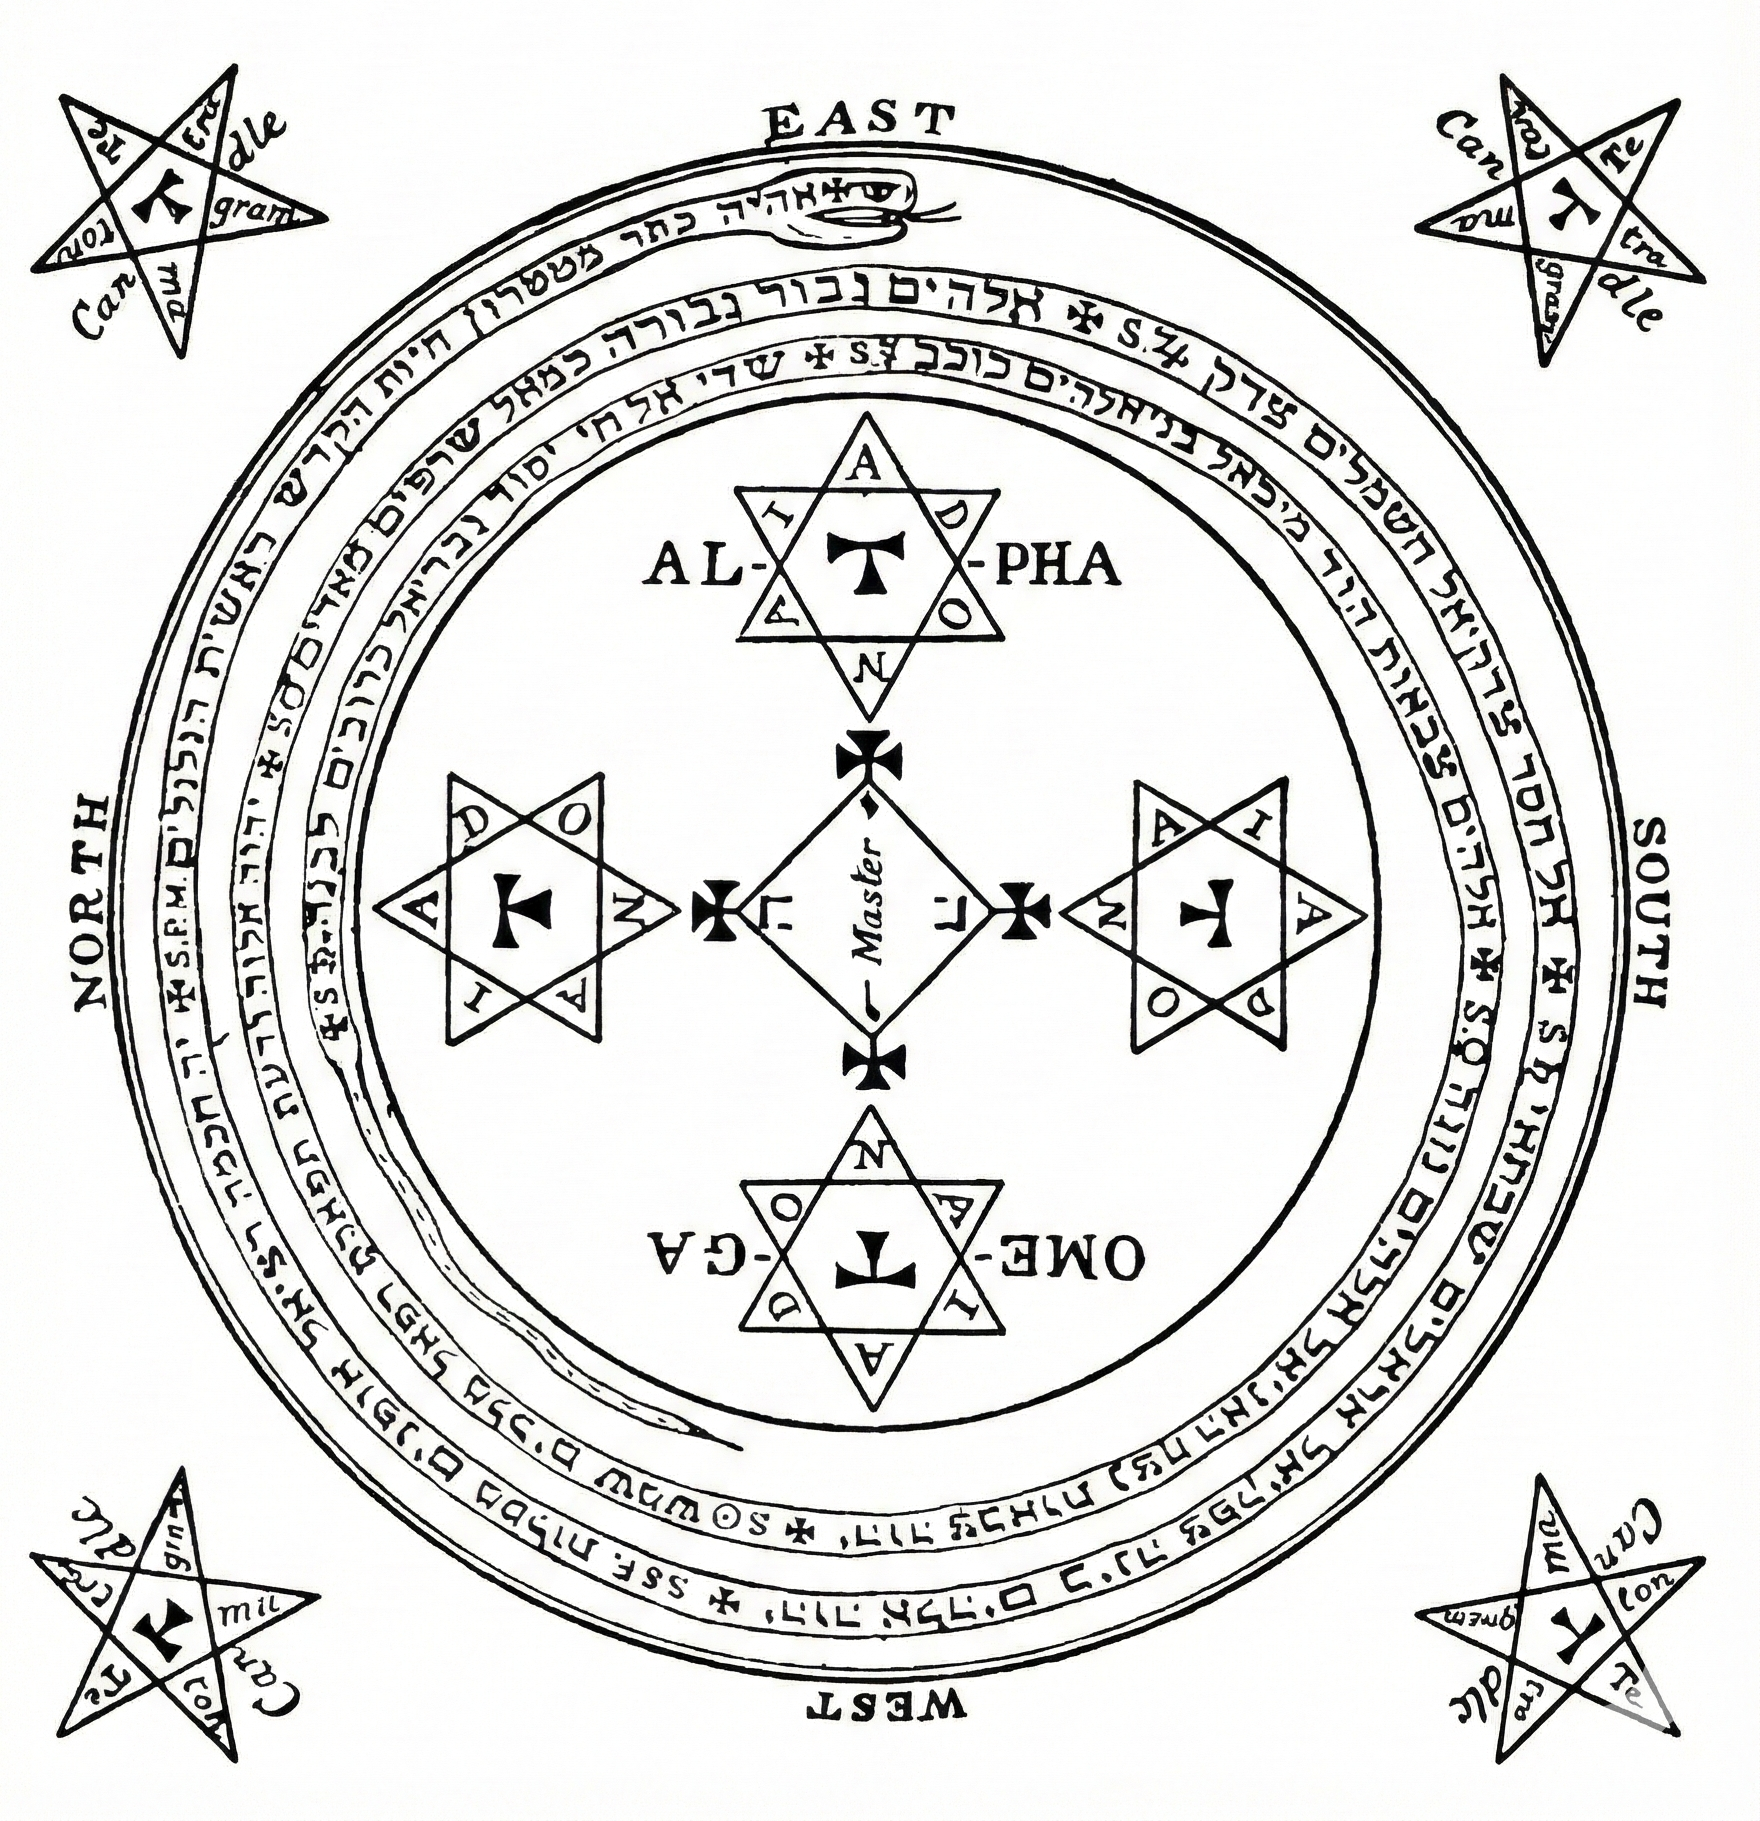
\includegraphics[width=0.3\paperwidth,keepaspectratio]{solomon_circle.png}
		\caption{The Circle of Solomon}
		\label{fig:solomoncircle}
	\end{figure}
	
	\subsection{The Triangle of Art (Repulsion Configuration)}
	For repulsion rather than summoning, the triangle's point faces OUTWARD from the protected space.  The three sides bear:
	\begin{figure}[H]
		\centering
		\includegraphics[width=0.3\paperwidth,keepaspectratio]{solomon_triangle.png}
		\caption{The Triangle of Art}
		\label{fig:solomontriangle}
	\end{figure}
	
	\begin{itemize}
		\item PRIMEUMATON (first moving)
		\item ANAPHAXETON (hidden one)
		\item TETRAGRAMMATON (the Name)
	\end{itemize}
	At the three points, inscribe MI-CHA-EL (Michael)---invoking the archangel who cast down rebellious spirits.  At center, place the Hexagram of Solomon containing no specific name, creating a \enquote{blank} binding that affects any entity.
	\begin{figure}[H]
		\centering
		\includegraphics[width=0.3\paperwidth,keepaspectratio]{solomon_hexagram.png}
		\caption{The Hexagram of Solomon}
		\label{fig:solomonhexagram}
		\cite[39]{mathersgoetia1904}
	\end{figure}
	
	\subsection{The Pentagram of Solomon}
	The most powerful generalized symbol in the system.  Originally worn by the magician for protection.
	\begin{figure}[H]
		\centering
		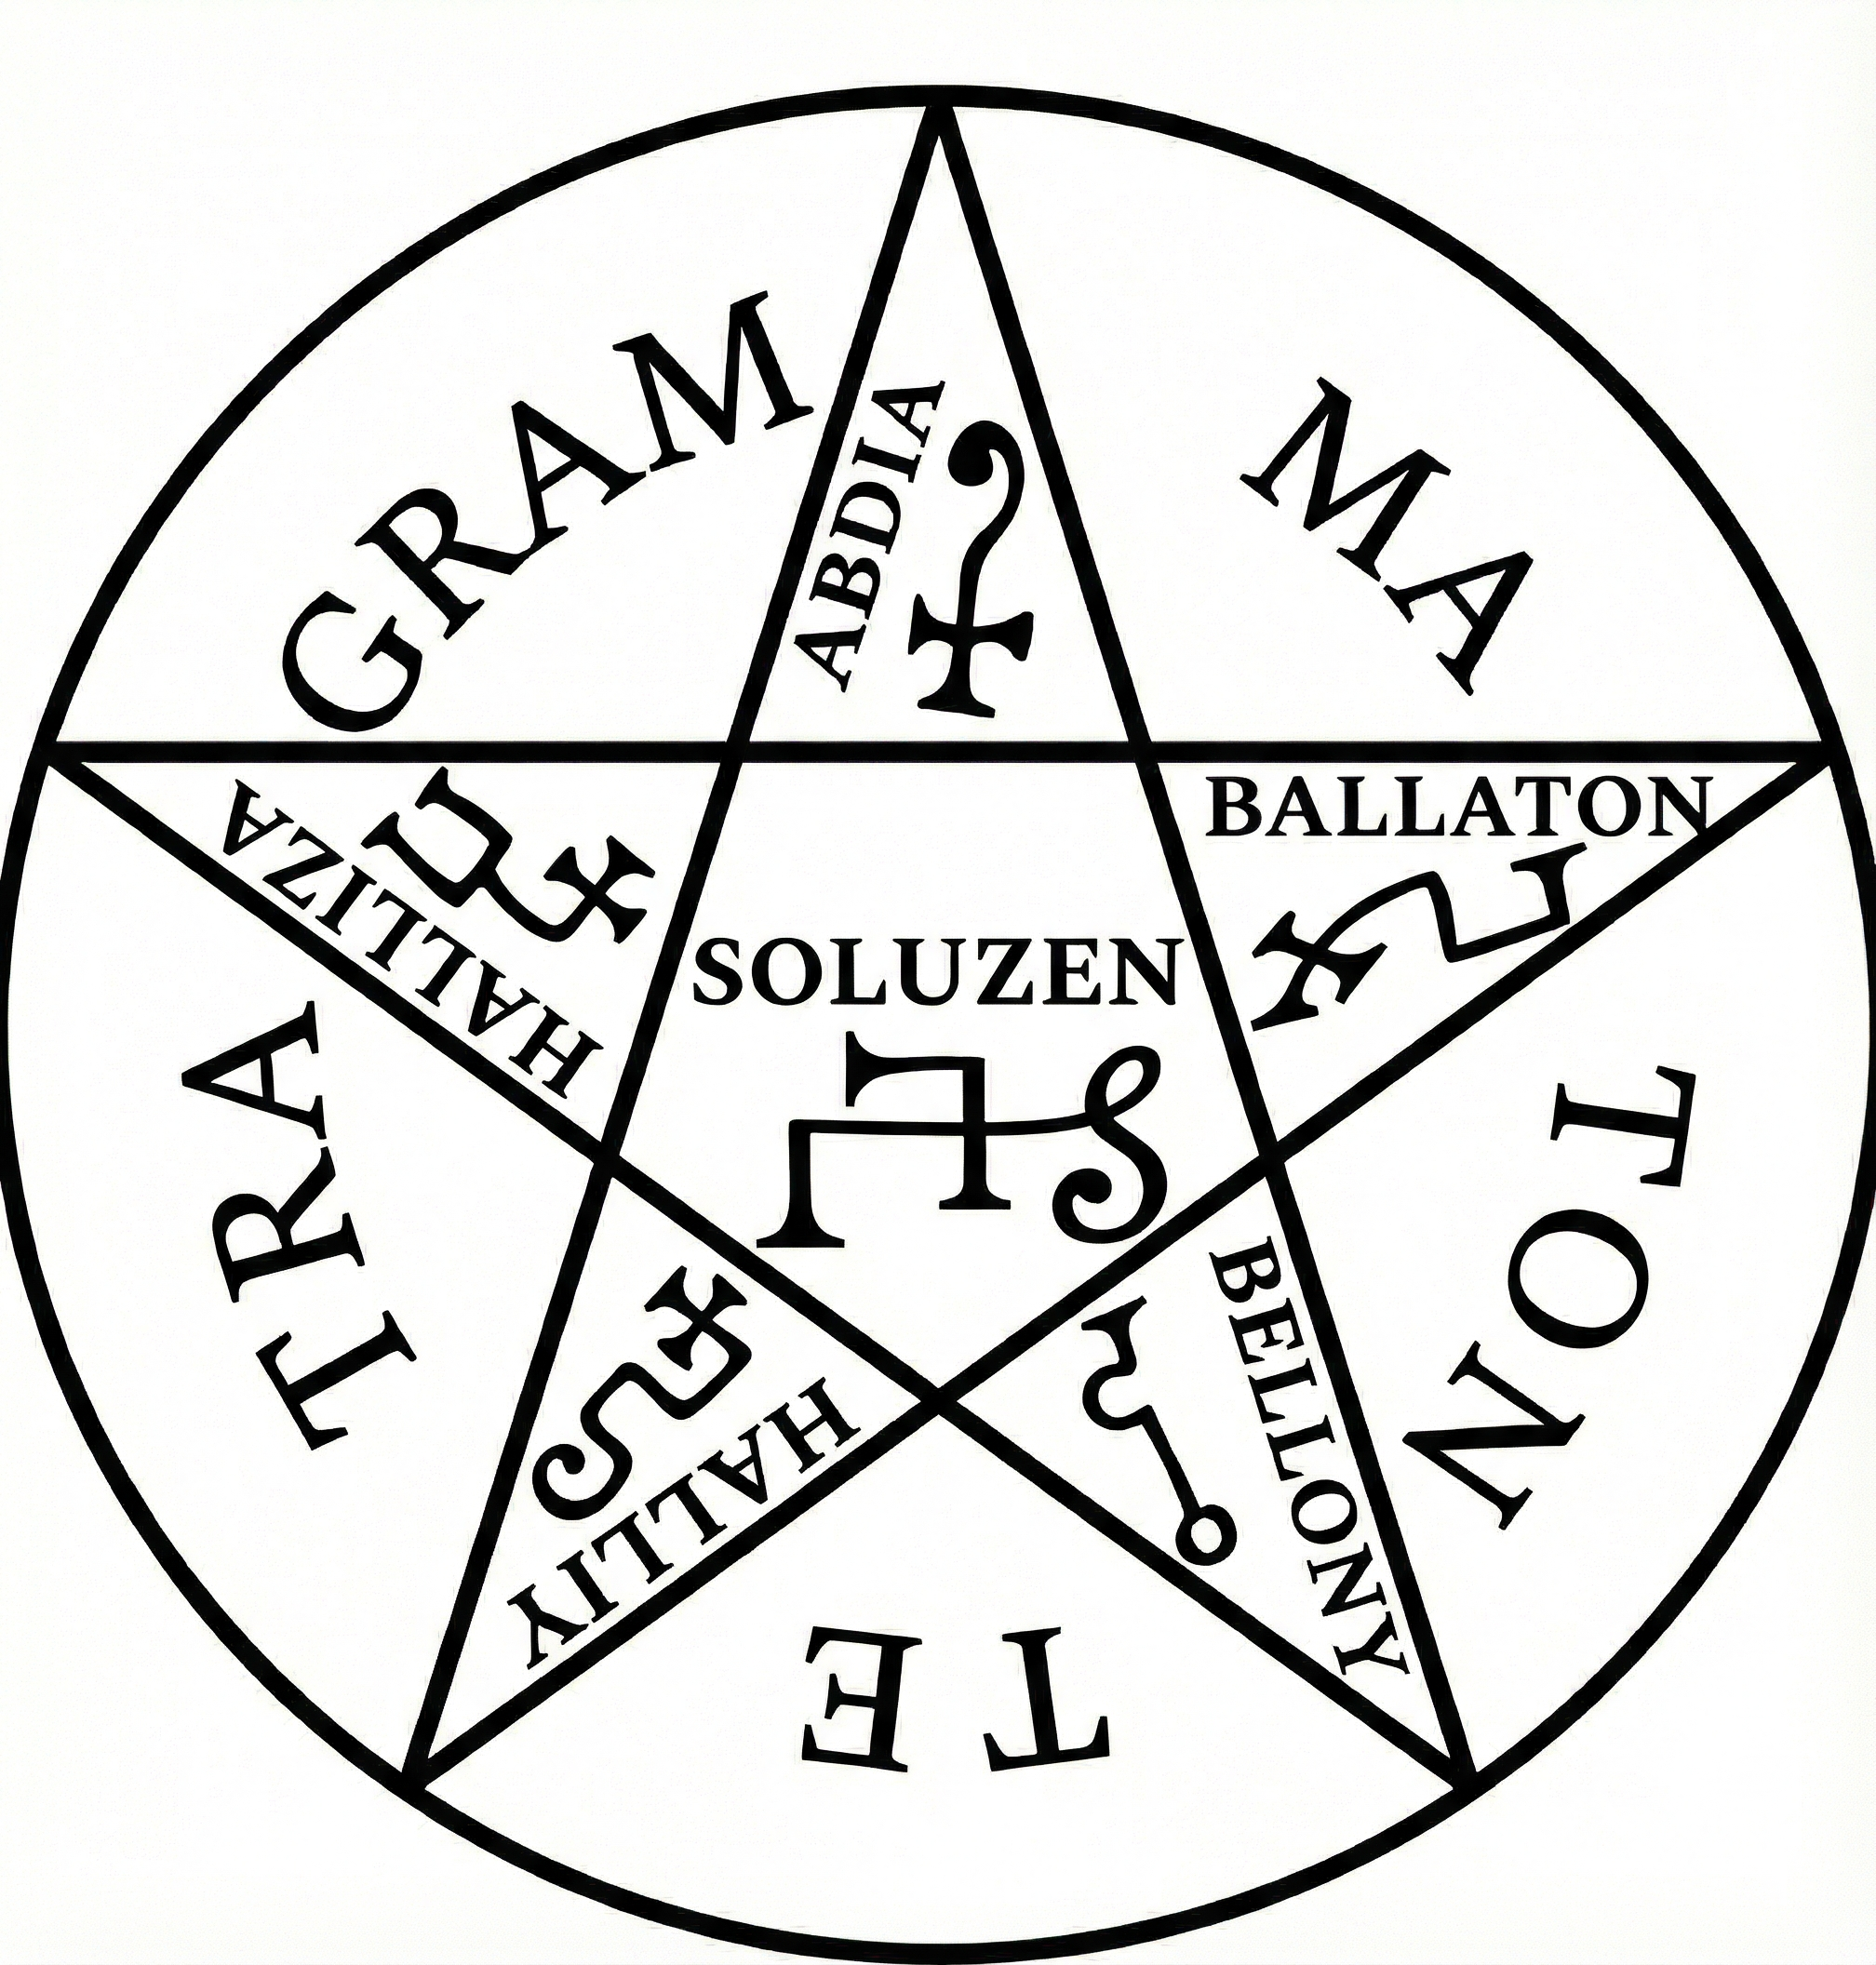
\includegraphics[width=0.3\paperwidth,keepaspectratio]{solomon_pentagram.png}
		\caption{The Pentagram of Solomon}
		\label{fig:solomonpentagram}
		\cite[39]{mathersgoetia1904}
	\end{figure}
	
	Elements:
	
	\begin{itemize}
		\item Five points: The five letters of YHShVH (Yahshuah---the \enquote{pentagrammaton})
		\item Center: The letters TE-TRA-GRAM-MA-TON arranged in the inner pentagon
		\item Outer ring: ABDIA, BALLATON, BELLONY, HALLIY, HALLIZA, SOLUZEN
	\end{itemize}
	For generalized repulsion: Inscribe on metal (traditionally copper or silver). Wear or mount at thresholds.  The symbol asserts authority over any of the 72 without needing to know which.
	
	\subsection{Combined Form}
	The union of the defensive circle and the constraining triangle creates the complete barrier.
	\begin{figure}[H]
		\centering
		\includegraphics[width=0.3\paperwidth,keepaspectratio]{solomon_circle_and_triangle.png}
		\caption[Circle and Triangle]{Circle and Triangle}
		\label{fig:circletriangle}
	\end{figure}

	\subsection{Spoken Formula for General Banishment}
	\begin{quotation}
	{\textquotedbl}By \gls{tetragrammaton}, ADONAI, AGLA, ON, EL---depart from this place.  By PRIMEUMATON who commands thy
	beginning and ANAPHAXETON who binds thy form---return to the depths appointed unto thee.{\textquotedbl}
	\end{quotation}
	
	
	\bigskip
	
	\clearpage

